\section{研究背景和动机}
这一节主要介绍研究的背景和研究的动机


\subsection{多核的普及与挑战}
随着多核机器的广泛普及,在可预见的未来,一个芯片上的CPU核数可以达到上百个,甚至千个\cite{borkar2007core}。
然而,如何简单并高效地利用多核资源依然是一个挑战,
因为并行编程依然是很困难的问题。
%如何简单有效地利用多核资源已成为一个十分重要的课题。
现有的多核上的并行编程模式,包括共享内存多线程pthread和消息传递MPI,
它们需要程序员自己手动的管理线程间的同步,负载的均衡,任务分派和调度等问题,
这要求程序员充分理解底层的硬件特性,
这无形中给程序员增加了很多负担,也让并行编程变得容易出错,且复杂。
为了让程序员避开这些设计的细节问题,一种可选的方案是依赖于运行时系统,让它管理所有这些并发的细节。


2004年Google提出了针对集群的MapReduce编程模型,极大的简化了并行编程\cite{dean2004mapreduce},
它以一种简单高效的方式执行大数据集的计算。
通过使用MapReduce模型,程序员不需要考虑复杂的底层设计,
只需要提供两个函数的实现:\kw{map()}和\kw{reduce()};
\kw{map()}函数处理输入数据集,并产生一系列的key-value对;
\kw{reduce}函数用于将具有相同key的多个value归并,得道最终的结果。

\subsection{Phoenix}
受到Google的MapReduce编程思想的启发,
耶鲁大学的Range等人将MapReduce编程模型移植到多核环境,
他们编写了一套针对多核的MapReduce库,
并通过实验证明,应用程序使用MapReduce编程模型在性能上可以与phtread编写的程序相媲美,
而且它延续了MapReduce的优点,就是它的编程接口简单
。用户可以不用熟悉多核环境,也不需要了解任务的分割和并行执行等问题,
只需要提供简单的map函数和reduce函数,就能够最大化的利用多核资源。
之后,为了让Phoenix能够获得更好的scalability,Yoo等人对Phoenix进行较大的改进和优化,
并提出了Phoenix2\cite{yoo2009phoenix2}(在本文中我们将其简称为Phoenix)。
其他的多核MapReduce库如Metis\cite{mao2010metis},
Tiled-mapreduce\cite{chen2010tiled},MRPhi\cite{lu2013mrphi}等,
都从各个角度对Phoenix进行优化。

\begin{figure}[!h!t]  
	\centering
	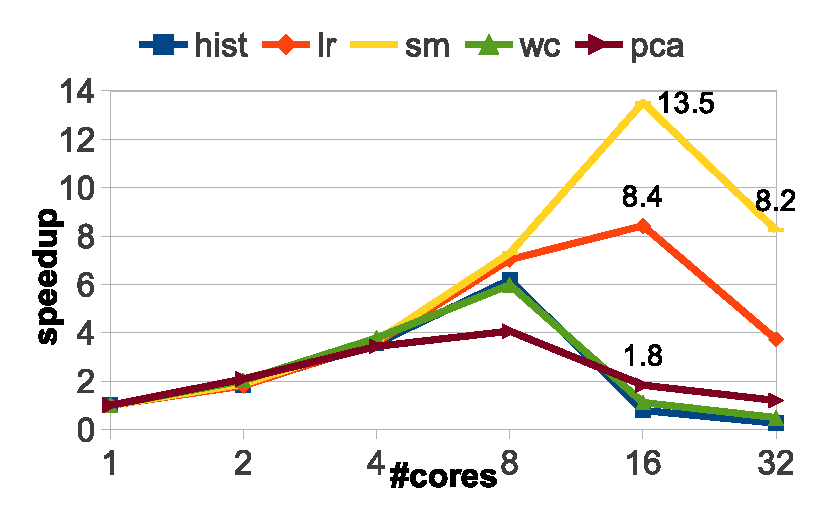
\includegraphics[width=0.5\textwidth]{eps/phoenix_speedup.eps}
	\caption{Speedup of workloads with Phoenix}
	\label{fig:phoenix:speedup}
\end{figure}


Phoenix利用基于共享内存的Pthreads库实现并发,
运行时系统中的每个worker会与一个Pthreads线程进行绑定。
理想情况下,向系统中增加更多的线程和核数,可以带来性能的提升,从而降低总的执行时间。
然而,实现的结果显示,Phoenix并不具有可伸缩性(实验的环境和配置细节将会在第\ref{sec:eval}节详细讲述)。
如图\ref{fig:phoenix:speedup}所示,各个MapReduce应用程序在Phoenix上的运行时间。
从实验结果可以看出,尽管Phoenix能够让应用程序并发的执行,
但是当核数超过16时,所有的应用程序的性能都开始变差。
事实上,当核数超过8使,大部分的应用程序的性能已经开始下降。
由此我们可以得出结论:多核环境下的Phoenix并不具有较好的scalability.

